\documentclass[11pt]{article}

\usepackage[margin=1in]{geometry}
\usepackage{mathptmx}
\usepackage{amsmath,amssymb}
\usepackage{booktabs}
\usepackage{threeparttable}
\usepackage{graphicx}
\usepackage{float}
\usepackage{caption}
\usepackage{enumitem}
\usepackage{url}
\usepackage[hidelinks]{hyperref}

\captionsetup{font=small,labelfont=bf,labelsep=period}
\setlength{\parindent}{0pt}
\setlength{\parskip}{6pt}
\renewcommand{\thesection}{\arabic{section}.}
\renewcommand{\thesubsection}{\thesection\arabic{subsection}.}
\renewcommand{\thesubsubsection}{\thesubsection\arabic{subsubsection}.}

\graphicspath{{../figures/}{figures/}}

\begin{document}

\begin{center}
{\Large\bfseries The Price of Bits: Privacy Shocks, Third-Party Data Dependence, and the Valuation of Digital Firms}
\end{center}

\vspace{0.2cm}

\begin{center}
Yile Wang $^{1,*}$\\
\vspace{0.15cm}
{\small $^{1}$ Affiliation, City, Country; email@example.com}\\
{\small $^{*}$ Correspondence: email@example.com}
\end{center}

\vspace{0.2cm}

\section*{Abstract}
\noindent
Data are a core production factor of the digital economy, yet their asset value lacks an observable market price. This paper exploits the 2021 Apple App Tracking Transparency (ATT) policy and China's Personal Information Protection Law (PIPL) as a privacy-regime shock. We construct a text-based Third-Party Data Dependency Index (TDDI) from the 2019 annual reports of 298 Chinese A-share digital firms and estimate difference-in-differences models on a firm-quarter panel from 2018Q1 to 2023Q4. Firms in the top third of TDDI experience a 9.2\% relative decline in log Tobin's Q and a 2.45 percentage-point decline in gross margin after the shock; ROA and selling-expense ratios do not change significantly. The effect is concentrated in B2B data-service firms, whereas consumer internet firms are not significantly affected. The implied market-value loss for high-exposure firms is RMB 203.7 billion (95\% CI: 54.7--352.8 billion). These findings quantify the firm-side value of third-party data and inform data-asset accounting and privacy-regulation policy.

\vspace{0.2cm}
\noindent\textbf{Keywords:} data asset valuation; privacy regulation; third-party data; difference-in-differences; text analysis; digital economy

\vspace{0.1cm}
\noindent\textbf{JEL Classification:} D22; K21; L86; M31; C23

\vspace{0.3cm}

\section{Introduction}
\label{sec:intro}

Data have become a defining production factor of the digital economy \cite{jones2020}. Unlike physical capital, data are non-rival: the same record can be reused across products, algorithms, and decisions without being depleted \cite{farboodi2020}. Their marginal replication cost is close to zero, so marginal cost provides little guidance for valuation \cite{bergemann2019}. Data are also rarely traded in transparent secondary markets, and their value is bundled with algorithms, platforms, and customer relationships \cite{oecd2022}. These features make firm-level data assets difficult to price.

Privacy regulation offers a way to observe the value of one class of data. The European Union's General Data Protection Regulation raised the cost of collecting and using personal data \cite{goldberg2024}. Apple's App Tracking Transparency (ATT) policy required user permission before cross-app tracking \cite{apple2020}. China's Personal Information Protection Law (PIPL) imposed consent, minimization, and sharing rules on personal information \cite{pipl2021}. A growing literature documents the effects of these regimes on e-commerce \cite{aridor2024}, app monetization \cite{kesler2023}, and the app ecosystem \cite{cheyre2024}.

Existing studies focus on average effects on outcomes. They do not measure how the value loss varies with a firm's ex ante dependence on third-party data. This distinction matters because digital firms differ sharply in their data architecture: some own logged-in users, transaction histories, and first-party applications, whereas others rely on external data purchases, cross-app identifiers, and platform traffic. A privacy shock should therefore have heterogeneous valuation effects even when it applies to all firms at the same time.

Measuring these differences is difficult because data use is not reported in financial statements. Text provides an alternative \cite{gentzkow2019}. Annual reports describe business models, traffic acquisition, advertising, data partnerships, and platform dependence \cite{loughran2011}. Dictionary-based text measures have been used to study policy uncertainty \cite{baker2016}, digital transformation \cite{jin2026}, and corporate disclosure \cite{loughran2011}. Building on this approach, we construct a Third-Party Data Dependency Index (TDDI) from the 2019 annual reports of Chinese A-share digital firms.

The TDDI covers four dimensions: third-party data acquisition, third-party traffic and advertising, user tracking and targeting, and platform dependence. We validate the index with split-half reliability, industry patterns, and a placebo index of generic digitalization. The index is predetermined relative to the 2021 privacy shock. This timing avoids the concern that firms adjust their disclosure in response to the regulation.

We combine the TDDI with a firm-quarter panel of 298 Chinese A-share digital firms from 2018Q1 to 2023Q4. We estimate difference-in-differences (DiD) models with firm and industry-by-quarter fixed effects \cite{dechaisemartin2020}. We report dynamic event studies \cite{rambachan2023}, dose-response bins \cite{callaway2024}, placebo dates, and wild cluster bootstrap inference \cite{mackinnon2017}. Identification rests on the timing of the privacy regime and on cross-sectional variation in pre-shock TDDI.

High-TDDI firms experience a 9.2\% relative decline in log Tobin's Q and a 2.45 percentage-point decline in gross margin after the shock. ROA and selling-expense ratios do not change significantly. The effect is concentrated in B2B data-service firms; consumer internet firms are not significantly affected. The implied market-value loss for high-exposure firms is RMB 203.7 billion, with a 95\% confidence interval of RMB 54.7--352.8 billion.

The paper makes four contributions. First, it provides a replicable, predetermined measure of third-party data dependence \cite{gentzkow2019}. Second, it estimates the valuation effect of a privacy-regime shock using a continuous exposure design \cite{aridor2024}. Third, it documents a B2B--B2C difference that is invisible in industry-average estimates \cite{chen2026}. Fourth, it translates the coefficient into a data risk exposure that can inform data-asset accounting and privacy policy \cite{ma2025}.

The research objectives are threefold. The first is to measure firm-level third-party data dependence from public disclosures. The second is to estimate how this dependence affects valuation and operating outcomes under the 2021 privacy regime. The third is to translate the estimates into an industry-level data risk exposure that can inform data-asset accounting and privacy policy.

The paper connects three literatures. The first treats data as an economic asset \cite{jones2020}. It emphasizes non-rivalry \cite{farboodi2020} and the market for information \cite{bergemann2019}. The second studies privacy and personalized markets \cite{acquisti2016}. It examines how consumers respond to tracking \cite{tucker2014} and how firms price privacy \cite{johnson2020}. The third uses text to measure firm-level digital and data characteristics \cite{gentzkow2019}. It also speaks to recent work in this journal on privacy regulation \cite{chen2026,li2026,kang2025,lin2021,zhang2026} and on the marketization of data elements in China \cite{jin2026,ma2025,song2025}.

The remainder of the paper proceeds as follows. Section 2 reviews the literature. Section 3 develops the theoretical analysis and states the hypotheses. Section 4 describes the institutional setting. Section 5 presents the data and sample. Section 6 constructs and validates the TDDI. Section 7 explains the empirical strategy. Section 8 reports the baseline results. Section 9 examines mechanisms and heterogeneity. Section 10 estimates the data risk exposure. Section 11 discusses implications, and Section 12 concludes.

\begin{figure}[H]
\centering
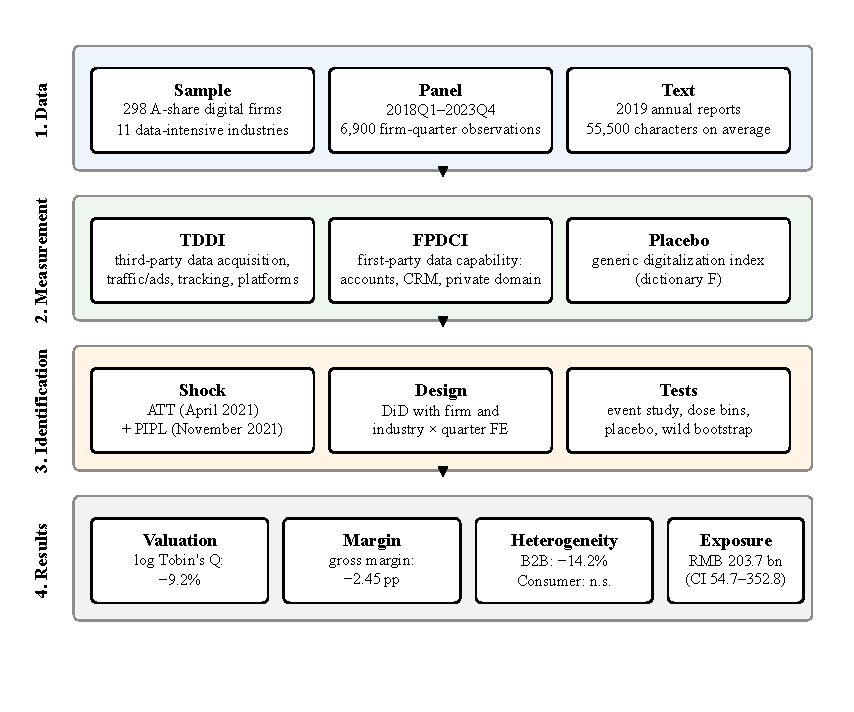
\includegraphics[width=0.95\textwidth]{fig0_framework.pdf}
\caption{Research framework. The figure summarizes the data, measurement, identification, and valuation steps. TDDI denotes the Third-Party Data Dependency Index; FPDCI denotes first-party data capability; DiD denotes difference-in-differences.}
\label{fig:framework}
\end{figure}

\section{Literature Review}
\label{sec:literature}

\subsection{Data as an Economic Asset}

The economics of data begins with the observation that data are non-rival. A single observation can be reused across many prediction problems without being consumed \cite{jones2020}. This property allows data to generate increasing returns at the level of the firm and the economy \cite{farboodi2020}. Data also differ from standard information goods because their value depends on the scale and scope of complementary algorithms, users, and organizational routines \cite{bergemann2019}. These features explain why data can be valuable even when no market price is observed.

Valuing data at the firm level is complicated by three measurement problems. First, most data are produced internally rather than purchased, so historical cost does not reflect economic value \cite{oecd2022}. Second, data are often combined with software, brands, and customer relationships, which makes it difficult to isolate a data-specific cash flow \cite{oecd2022}. Third, data are rarely traded in transparent secondary markets, so market-comparable prices are scarce \cite{bergemann2019}. The accounting literature has therefore turned to indirect approaches, such as the value of data-intensive business models or the response of firm value to data-related shocks.

China's data-element market provides a useful laboratory for these questions. The establishment of data trading platforms has been associated with changes in corporate innovation \cite{song2025} and investment efficiency \cite{ma2025}. These studies show that data marketization can affect real corporate outcomes, but they do not observe the shadow value of a particular data input at the firm level. Our paper complements this work by using a privacy shock to recover the value of one narrowly defined data input: third-party tracking and advertising data.

\subsection{Privacy, Personalization, and Regulation}

A large literature studies how privacy shapes consumer behavior and market outcomes. Consumers face a trade-off between the benefits of personalization and the costs of information disclosure \cite{acquisti2016}. Their privacy concerns are context-dependent and can shift with experience and salience \cite{acquisti2015}. Privacy concerns also respond to salient public events and regulatory attention \cite{goldfarb2012}. Field evidence shows that privacy controls affect the demand for personalized advertising \cite{tucker2014} and that opt-out choices vary systematically across consumers \cite{johnson2020}. Personalized advertising can improve match quality \cite{bleier2015}, but its effectiveness depends on the credibility and transparency of the data practice \cite{boerman2017}.

Firms also choose privacy as a competitive dimension. A firm may compete by offering stronger privacy protection to attract privacy-sensitive consumers \cite{casadesus2015}. Price discrimination based on purchase history can raise profits but may trigger consumer backlash \cite{acquisti2005}. When consumers can disclose information strategically, the equilibrium amount of disclosure depends on the market structure and the value of personalization \cite{ichihashi2020}. Consumer scores and scoring technologies further complicate the welfare effects of data collection \cite{bonatti2020}.

Information systems research emphasizes the antecedents and consequences of privacy concerns. Perceived fairness and trust shape consumers' willingness to disclose information \cite{culnan1999,dinev2006}. Privacy concerns are multidimensional, and their effect on behavior depends on the perceived benefits and risks of disclosure \cite{malhotra2004}. Legal and normative scholarship debates whether privacy should be treated as a property right, a dignitary interest, or a contextual norm \cite{nissenbaum2009,samuelson2000}. The economic analysis of privacy as secrecy shows that the efficiency of disclosure depends on the allocation of property rights \cite{hermalin2006}.

Privacy regulation changes the equilibrium of these markets. The GDPR reduced the intensity of online tracking and shifted traffic and revenue toward larger publishers \cite{goldberg2024}. Earlier evidence from the GDPR documents heterogeneous effects across firms and websites \cite{aridor2020}. Apple's ATT policy reduced advertising effectiveness and app monetization \cite{aridor2024,kesler2023}, with downstream effects on the app ecosystem \cite{cheyre2024}. Recent work in this journal examines opt-in versus inference regulation \cite{li2026}, users' data sharing under privacy protection \cite{kang2025}, the welfare effects of privacy regulation \cite{lin2021}, retailer resilience under privacy regulation \cite{chen2026}, and the privacy--personalization paradox on content platforms \cite{zhang2026}. Related work studies the regulation of data abuse on digital platforms \cite{wang2023} and the governance of privacy--personalization tension in customer data platforms \cite{mihaylova2026}.

These studies establish that privacy regulation has real economic effects. They do not, however, quantify how the effect varies with a firm's ex ante dependence on third-party data. Most designs compare regulated and unregulated markets, or users who are exposed to a consent prompt and those who are not. The cross-sectional variation that matters for asset valuation—why some firms lose more value than others within the same regulated market—remains largely unexplored.

\subsection{Measuring Firm-Level Data Dependence}

Text is a natural source for measuring firm-level data practices. Computational text analysis has become a standard tool in economics and finance \cite{gentzkow2019}. Dictionary methods can recover economically meaningful variation from corporate disclosures \cite{loughran2011}. Text-based measures have been used to study policy uncertainty \cite{baker2016}, digital transformation \cite{jin2026}, and the tone of corporate communication \cite{loughran2011}. These measures are replicable, transparent, and available for large samples.

Existing text measures capture the intensity of digitalization, not the structure of data dependence. A firm that invests heavily in cloud computing, artificial intelligence, and digital channels may rely mostly on first-party data. A firm that buys traffic, uses third-party audiences, and depends on platform interfaces may be data-intensive in a different sense. The distinction matters for privacy regulation: the former can substitute first-party data for external data, whereas the latter cannot. We therefore construct an index that targets third-party data dependence directly.

\subsection{Hypotheses Development}

We derive four hypotheses from the theory in Section 3 and the empirical evidence reviewed above.

\textit{H1 (Valuation effect).} After the privacy shock, firms with higher pre-shock TDDI experience a larger decline in Tobin's Q. The mechanism is a reduction in the expected rents from third-party data. The market value of a firm is the present value of future profits; when the data input becomes more costly or less usable, the present value falls. The decline should be larger for firms whose production function has a higher elasticity with respect to third-party data.

\textit{H2 (Operating effect).} After the shock, high-TDDI firms experience a decline in gross margin, while ROA may not change significantly in the short run. Third-party data affect pricing, targeting, and conversion. A reduction in data availability lowers the revenue per unit of cost, which shows up in gross margin. Firms can cut low-efficiency marketing and administrative spending, which buffers ROA. The prediction is therefore a decline in gross margin without a commensurate decline in ROA.

\textit{H3 (B2B versus B2C heterogeneity).} The valuation effect is concentrated in B2B data-service firms rather than consumer internet firms. B2B data-service firms (IT services, software, and communication services) obtain data through external purchases, client authorization, and cross-organizational sharing. Consumer internet firms (advertising, gaming, e-commerce, and content platforms) own user accounts, transaction records, and first-party applications. First-party data can substitute for third-party data in consumer firms, but less so in B2B data-service firms.

\textit{H4 (First-party data moderation).} The moderating role of first-party data capability (FPDCI) is theoretically ambiguous. If first-party and third-party data are substitutes, high-FPDCI firms should be less affected by the shock. If they are complements—high-FPDCI firms also use large amounts of external data to extend coverage and improve models—the moderation may be zero or even negative. We therefore treat H4 as an open empirical question rather than a one-sided prediction.
The literature establishes three facts. Data are economically valuable but difficult to price at the firm level. Privacy regulation changes the availability and cost of personal data. Text can recover firm-level data practices from public disclosures. What remains missing is a measure that separates third-party data dependence from generic digitalization and a design that links this measure to firm value under a privacy shock. This paper fills that gap by constructing the TDDI and by estimating its valuation effect around the 2021 privacy regime.

\section{Theoretical Analysis}
\label{sec:theory}

\subsection{Production with First- and Third-Party Data}

Consider a firm $i$ that produces output $Y_{it}$ using physical capital $K_{it}$, labor $L_{it}$, first-party data $D^{1}_{it}$, and third-party data $D^{3}_{it}$. The production function is
\begin{equation}
Y_{it}=A_{it}K_{it}^{\alpha}L_{it}^{\beta}\left(D^{1}_{it}\right)^{\gamma_1}\left(D^{3}_{it}\right)^{\gamma_3},
\label{eq:production}
\end{equation}
with $\alpha,\beta,\gamma_1,\gamma_3>0$ and $\alpha+\beta+\gamma_1+\gamma_3<1$. First-party data are accumulated through the firm's own users, transactions, and applications. Third-party data are purchased or accessed through external vendors, advertising networks, identifiers, and platform interfaces at unit cost $p_3$.

The firm chooses $K$, $L$, and $D^3$ to maximize profit,
\begin{equation}
\pi_{it}=Y_{it}-wL_{it}-rK_{it}-p_3D^{3}_{it}.
\label{eq:profit}
\end{equation}
The first-order condition for third-party data is
\begin{equation}
\frac{\gamma_3Y_{it}}{D^{3}_{it}}=p_3,
\label{eq:foc}
\end{equation}
which implies $D^{3}_{it}=\gamma_3Y_{it}/p_3$. Substituting back into \eqref{eq:production} gives
\begin{equation}
Y_{it}=\left[A_{it}K_{it}^{\alpha}L_{it}^{\beta}\left(D^{1}_{it}\right)^{\gamma_1}\left(\frac{\gamma_3}{p_3}\right)^{\gamma_3}\right]^{\frac{1}{1-\gamma_3}}.
\label{eq:reduced}
\end{equation}
Output and profit are increasing in the productivity of third-party data, $\gamma_3$, and decreasing in its cost, $p_3$.

\subsection{The Privacy Shock and Firm Value}

The 2021 privacy regime raises the effective cost of third-party data. We model the shock as a reduction in the usable stock of third-party data:
\begin{equation}
D^{3,\text{post}}_{it}=(1-\phi_i)D^{3,\text{pre}}_{it},
\label{eq:shock}
\end{equation}
where $\phi_i\in(0,1)$ is the exposure of firm $i$. The exposure is larger for firms whose business model relies more heavily on external data. The TDDI is a proxy for $\phi_i$.

For a fixed capital stock and labor input, output after the shock is
\begin{equation}
Y^{\text{post}}_{it}=(1-\phi_i)^{\gamma_3}Y^{\text{pre}}_{it}.
\label{eq:outputshock}
\end{equation}
Firm value is the present value of profits, $V_{it}=E_t\sum_{\tau=0}^{\infty}\delta^{\tau}\pi_{i,t+\tau}$. For small $\phi_i$, the proportional change in firm value is
\begin{equation}
\frac{\partial\ln V_{it}}{\partial\phi_i}\approx-\gamma_3.
\label{eq:value}
\end{equation}
Because Tobin's Q is $Q_{it}=V_{it}/A_{it}$ and the asset base is predetermined in the short run, the valuation effect is
\begin{equation}
\frac{\partial\ln Q_{it}}{\partial\phi_i}\approx-\gamma_3<0.
\label{eq:q}
\end{equation}
The effect is larger when the output elasticity of third-party data, $\gamma_3$, is higher. Since TDDI is increasing in the firm's reliance on third-party data, \eqref{eq:q} yields the first hypothesis.

\textit{H1 (Valuation effect).} High-TDDI firms experience a larger decline in Tobin's Q after the privacy shock.

\subsection{Gross Margin and Accounting Profit}

The production model treats output price as fixed. In digital markets, third-party data also affect the price that consumers are willing to pay and the efficiency of matching. Let $P_{it}(D^{3}_{it})$ be the unit price, with $P'(\cdot)>0$: better targeting and measurement raise the value of the product to consumers. Let $c$ be the unit cost. The gross margin is
\begin{equation}
GM_{it}=1-\frac{c}{P_{it}\left(D^{3}_{it}\right)}.
\label{eq:gm}
\end{equation}
Differentiating with respect to $D^{3}_{it}$ gives
\begin{equation}
\frac{\partial GM_{it}}{\partial D^{3}_{it}}=\frac{cP'_{it}\left(D^{3}_{it}\right)}{P_{it}^{2}}>0.
\label{eq:gmderiv}
\end{equation}
A reduction in third-party data lowers the price premium and therefore lowers the gross margin. ROA can respond less because firms cut low-productivity marketing and administrative spending, and because the asset base adjusts slowly. This yields the second hypothesis.

\textit{H2 (Operating effect).} High-TDDI firms experience a decline in gross margin after the shock, while the short-run ROA effect is smaller or statistically insignificant.

\subsection{B2B versus B2C Firms}

The model also implies heterogeneity across business models. Let $\gamma_3/(\gamma_1+\gamma_3)$ be the share of data-related output elasticity attributable to third-party data. B2B data-service firms sell data-intensive services to other firms and obtain data through external purchases, client authorization, and cross-organizational sharing. Their $\gamma_3$ is high and their $D^{1}$ is limited. Consumer internet firms own user accounts, transaction histories, and first-party applications; their $D^{1}$ is high and can substitute for $D^{3}$. The same privacy shock therefore produces a larger valuation decline for B2B data-service firms. This yields the third hypothesis.

\textit{H3 (B2B versus B2C heterogeneity).} The negative valuation effect is concentrated in B2B data-service firms and is weaker or absent in consumer internet firms.

\subsection{First-Party Data as a Substitute or Complement}

To formalize the role of first-party data, suppose that the two data inputs enter through a CES aggregator:
\begin{equation}
D_{it}=\left[\kappa\left(D^{1}_{it}\right)^{\rho}+(1-\kappa)\left(D^{3}_{it}\right)^{\rho}\right]^{1/\rho},
\label{eq:ces}
\end{equation}
where $\rho\leq1$ and the elasticity of substitution is $\sigma=1/(1-\rho)$. If $\rho>0$, the two data types are substitutes: a firm with abundant first-party data can replace part of the lost third-party data, and the valuation effect is smaller for high-FPDCI firms. If $\rho<0$, the two data types are complements: first-party data increase the return to third-party data, and high-FPDCI firms may be equally or more exposed. The sign of the moderation is therefore an empirical question. This yields the fourth hypothesis.

\textit{H4 (First-party data moderation).} The moderating effect of FPDCI on the valuation effect can be positive (substitutes) or zero/negative (complements).

\subsection{From Theory to the Estimating Equation}

Combining \eqref{eq:q} with the definition of the shock, the log valuation of firm $i$ in quarter $t$ can be written as
\begin{equation}
\ln Q_{it}=\alpha_i+\lambda_{s(i)t}-\beta\left(\text{HighTDDI}_i\times\text{Post}_t\right)+\Gamma'X_{it}+\varepsilon_{it},
\label{eq:empirical}
\end{equation}
where $\alpha_i$ is a firm fixed effect, $\lambda_{s(i)t}$ is an industry-by-quarter fixed effect, $\text{Post}_t$ indicates the post-2021Q3 period, and $\beta$ is proportional to the average $\gamma_3\phi_i$ of high-TDDI firms. The coefficient $\beta$ is the object of the empirical analysis. The model also implies that a continuous TDDI specification should yield a negative coefficient and that the effect should be larger for firms with a higher share of third-party data in production.

Equation~\eqref{eq:empirical} is a reduced-form valuation effect. It combines the direct loss of third-party data with firms' adaptation through first-party data, contextual advertising, and cost reduction, which is the object relevant for asset valuation. ATT and PIPL operate through different margins---consent, measurement, and sharing---and the design estimates their combined effect on firm value.

\section{Institutional Background: The 2021 Privacy Regime}
\label{sec:institution}

\subsection{Apple App Tracking Transparency}

Apple announced ATT at its Worldwide Developers Conference in June 2020. The policy took effect with the release of iOS 14.5 on 26 April 2021. Under ATT, an app must obtain explicit user permission before tracking a user across other companies' apps and websites or accessing the advertising identifier. If a user declines, the app receives a zeroed identifier and cannot conduct user-level attribution, retargeting, or lookalike-audience construction across apps \cite{apple2020}. ATT therefore changed the default rules of the mobile advertising market: cross-app tracking moved from opt-out to opt-in.

The economic consequences of ATT have been documented in several markets. ATT reduced advertising effectiveness and sales for e-commerce firms \cite{aridor2024}. It lowered app monetization for developers \cite{kesler2023}. It also changed competition and entry in the app ecosystem \cite{cheyre2024}. These findings establish that ATT is a substantive shock to the third-party data ecosystem, not a narrow technical change.

\subsection{China's Personal Information Protection Law}

China's PIPL was adopted on 20 August 2021 and took effect on 1 November 2021. The law establishes a legal basis for processing personal information, requires informed consent for sensitive information and cross-border transfers, and imposes minimization and accountability obligations on data controllers \cite{pipl2021}. The Data Security Law, effective 1 September 2021, introduced data classification and security assessment rules for important data and cross-border data flows \cite{dsl2021}. Together, the two laws raised the cost of acquiring, sharing, and using third-party personal data.

For Chinese digital firms, the 2021 regime is a combined shock. ATT cut the default supply of cross-app identifiers on Apple devices. PIPL and the Data Security Law raised the legal and compliance cost of using personal data on all devices. The two shocks are adjacent in time and complementary in mechanism. We therefore define 2021Q3 as the first post-shock quarter: ATT had taken effect at the end of Q2, and firms began adjusting their data, advertising, and compliance practices in Q3. Figure \ref{fig:timeline} summarizes the timeline.

\subsection{Why 2021 Is a Useful Shock}

The 2021 regime has three features that make it useful for identification. First, the timing was set by Apple and by the Chinese legislature, not by individual firms. A single A-share firm could not choose the implementation date or the content of the rules. Second, the shock changed the availability and cost of third-party data without directly changing firms' physical capital, labor, or product markets. Third, the shock had differential intensity: firms with different ex ante data architectures were exposed to different degrees. The identifying variation is therefore a common shock interacted with predetermined firm-level exposure.

The design does not isolate the effect of ATT from the effect of PIPL. Instead, it estimates the combined effect of the 2021 privacy regime on firms with different third-party data dependence. This is the relevant object for asset valuation: investors price the net effect of the regime, not the effect of a single statute. The next sections describe how we measure exposure and how we estimate its valuation effect.

\begin{figure}[htbp]
\centering
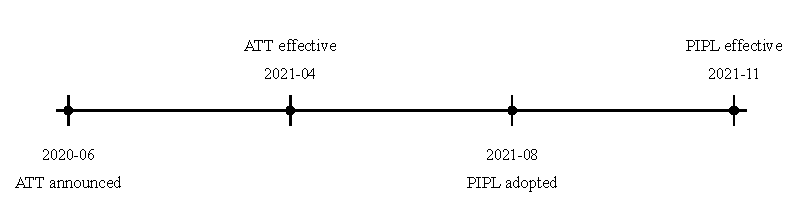
\includegraphics[width=0.95\textwidth]{fig1_timeline.pdf}
\caption{Timeline of the 2021 privacy regime. ATT was announced in June 2020 and took effect with iOS 14.5 in April 2021. PIPL was adopted in August 2021 and implemented in November 2021. The empirical analysis defines 2021Q3 as the first post-shock quarter.}
\label{fig:timeline}
\end{figure}

\section{Data and Sample}
\label{sec:data}

\subsection{Sample Construction}

The sample frame consists of Chinese A-share firms in 11 data-intensive industries: IT services, software development, communication services, advertising and marketing, publishing, gaming, education, film and cinema, internet e-commerce, digital media, and broadcasting. These industries cover the main segments of the digital economy, including e-commerce, digital media, advertising, data services, and platform-mediated transactions. In 2021Q1, the frame contained 384 non-ST, non-delisted firms.

We construct the sample in three steps. First, we exclude firms that listed after 2019 and therefore lack a 2019 annual report, as well as firms whose annual-report files are unavailable; this removes 86 firms. Second, we retain firms with a parseable 2019 annual report and complete financial and market data, leaving 298 firms. Third, we use quarterly observations from 2018Q1 to 2023Q4. The final panel contains 6,900 firm-quarter observations, with 3,933 pre-shock and 2,967 post-shock observations. Table \ref{tab:desc} reports the sample construction and descriptive statistics.

\subsection{Data Sources and Variables}

Financial statement data are from the Eastmoney data center. The data include total assets, total liabilities, total equity, cash holdings, operating revenue, operating costs, selling expenses, administrative expenses, operating profit, and net profit attributable to the parent. Market capitalization is the total market value at the last trading day of each quarter, also from Eastmoney; when the market value is missing, we infer it from the price-to-book ratio multiplied by book equity. Stock price and index data from Sina Finance are used to cross-check quarter-end market values. Annual-report texts are from the CNINFO and Eastmoney disclosure platforms.

Tobin's Q is defined as the sum of equity market value and total liabilities divided by total assets. Log Tobin's Q is its natural logarithm. ROA is net profit divided by total assets. Gross margin is operating revenue minus operating costs, divided by operating revenue. The selling-expense ratio is selling expenses divided by operating revenue; the period-expense ratio is the sum of selling and administrative expenses divided by operating revenue. Firm size is the natural logarithm of total assets; leverage is total liabilities divided by total assets; the cash ratio is cash holdings divided by total assets. All ratio variables are winsorized at the 1st and 99th percentiles.

Quarterly flow variables are obtained by differencing year-to-date cumulative items. Q1 equals the cumulative Q1 value; Q2 equals the half-year value minus Q1; Q3 equals the nine-month value minus the half-year value; Q4 equals the annual value minus the nine-month value. This conversion removes seasonality from cumulative reporting and makes ROA, gross margin, and expense ratios comparable across quarters. Observations with missing intermediate quarters are treated as missing rather than interpolated. Appendix Table 
ef{tab:vars} lists variable definitions and sources.

\subsection{Descriptive Statistics}

Panel B of Table \ref{tab:desc} reports the descriptive statistics. The average Tobin's Q is 2.80, and the average log Tobin's Q is 0.86. The average ROA is 0.3\%, the average gross margin is 36.0\%, the average selling-expense ratio is 11.7\%, and the average period-expense ratio is 23.1\%. Between the pre- and post-shock periods, Tobin's Q declines from 2.96 to 2.60, log Tobin's Q from 0.90 to 0.81, and gross margin from 37.2\% to 34.4\%. These raw differences mix the privacy shock with macroeconomic conditions, industry cycles, and compositional changes; they provide magnitudes, not causal effects.

The high-TDDI group contains 100 firms, and the remaining 198 firms form the comparison group. The high-TDDI firms had a combined equity market value of RMB 1.72 trillion in 2021Q1, or 46\% of the sample total. Third-party data dependence is therefore not a marginal phenomenon in the Chinese digital capital market. The industry distribution and the TDDI distribution appear in Section 6 and Figure \ref{fig:tddi}.

\begin{table}[htbp]
\centering
\small
\caption{Sample construction and descriptive statistics.}
\label{tab:desc}
\begin{threeparttable}
\begin{tabular}{lcccc}
\toprule
 & Full sample & SD & Pre-shock & Post-shock \\
\midrule
\multicolumn{5}{l}{Panel A: Sample construction} \\
Firms in the 11 digital industries (2021Q1) & 384 & & & \\
\quad Less: no usable 2019 annual report & 86 & & & \\
\quad Final sample & 298 & & & \\
Firm-quarter observations & 6{,}900 & & 3,933 & 2,967 \\
High-TDDI firms & 100 & & & \\
\midrule
\multicolumn{5}{l}{Panel B: Main variables} \\
Log Tobin's Q & 0.861 & 0.558 & 0.901 & 0.809 \\
Tobin's Q & 2.804 & 1.899 & 2.960 & 2.597 \\
ROA & 0.003 & 0.037 & 0.006 & -0.000 \\
Gross margin & 0.360 & 0.231 & 0.372 & 0.344 \\
Selling-expense ratio & 0.117 & 0.121 & 0.115 & 0.120 \\
Period-expense ratio & 0.231 & 0.172 & 0.228 & 0.235 \\
Revenue growth & 0.123 & 0.534 & 0.174 & 0.073 \\
Firm size & 22.028 & 1.033 & 21.996 & 22.071 \\
Leverage & 0.361 & 0.192 & 0.347 & 0.378 \\
Cash ratio & 0.212 & 0.146 & 0.210 & 0.214 \\
TDDI & 0.001 & 0.998 & -0.001 & 0.004 \\
FPDCI & 0.008 & 1.003 & 0.011 & 0.004 \\
\bottomrule
\end{tabular}
\begin{tablenotes}[flushleft]
\footnotesize
\item Notes: All ratio variables are winsorized at the 1st and 99th percentiles. Pre-shock is 2018Q1--2021Q2; post-shock is 2021Q3--2023Q4. TDDI and FPDCI are standardized to mean zero and unit standard deviation. Firm size is the natural logarithm of total assets.
\end{tablenotes}
\end{threeparttable}
\end{table}


\section{Measuring Third-Party Data Dependence}
\label{sec:measurement}

\subsection{Text Corpus}

The text corpus consists of the 2019 annual reports of the sample firms. We use annual reports rather than earnings-call transcripts for three reasons. First, annual reports follow a standardized disclosure format and cover the full sample; earnings-call transcripts for Chinese digital firms are incomplete in 2019. Second, the ``Business Overview'' and ``Management Discussion and Analysis'' sections describe business models, customer structure, traffic sources, advertising, data partnerships, and platform dependence, which map directly to the four dimensions of third-party data dependence. Third, the 2019 reports were published in early 2020, before ATT and PIPL, and are therefore predetermined with respect to the shock.

For each PDF, we locate the main body of the business overview or management discussion section and retain a 60,000-character window. We remove page headers, footers, and page numbers. If a firm uses a different heading, we use the main-text start as the anchor. The final corpus contains 298 parseable reports with an average length of about 55,500 characters.

\subsection{Lexicon and Index Construction}

The lexicon has six categories. Category A covers third-party data acquisition, including ``third-party data'', ``purchased data'', ``data procurement'', ``data supplier'', ``data transaction'', ``data sharing'', and ``data interface''. Category B covers third-party traffic and advertising, including ``traffic purchase'', ``customer acquisition cost'', ``ad buying'', ``advertising placement'', ``precision marketing'', ``programmatic advertising'', ``information-flow advertising'', ``ad network'', and ``app distribution''. Category C covers user profiling and tracking, including ``user profile'', ``tag system'', ``cross-app'', ``cross-device'', ``device identifier'', ``IDFA'', ``OAID'', ``targeted placement'', and ``personalized recommendation''. Category D covers platform dependence, including ``third-party platform'', ``open platform'', ``app store'', ``iOS'', ``WeChat mini-program'', ``Douyin'', ``Kuaishou'', ``Xiaohongshu'', ``Ocean Engine'', and ``Alimama''. Category E covers first-party data capability, including ``owned data'', ``first-party data'', ``private-domain traffic'', ``membership system'', ``user community'', ``WeCom'', ``CRM'', ``data middle platform'', and ``CDP''. Category F covers generic digitalization, including ``digital transformation'', ``cloud computing'', ``big data'', ``artificial intelligence'', ``Internet of Things'', ``blockchain'', ``5G'', ``industrial internet'', and ``large language model''.

Term counts use a longest-match rule: within a character span, the longest term is matched first, so nested terms such as ``data service'' and ``data service provider'' are not double counted. Let $N_{ic}$ be the count of category $c$ for firm $i$ and $L_i$ the text length. The category intensity is $10{,}000\times N_{ic}/L_i$. The TDDI is the equal-weighted average of the four treatment categories, log-transformed and standardized:
\begin{equation}
\text{TDDI}_i=\text{Std}\left[\ln\left(1+\frac{1}{4}\sum_{c=A}^{D}\frac{10{,}000N_{ic}}{L_i}\right)\right].
\label{eq:tddi}
\end{equation}
Equal weighting prevents categories with more terms from dominating the index. The log transformation limits the influence of a small number of firms with very high disclosure frequency. FPDCI and the generic digitalization index are constructed in the same way from categories E and F. Appendix Table 
ef{tab:lexicon} lists the six constructs and representative terms.

\subsection{Reliability and Construct Validity}

Table \ref{tab:validity} reports the reliability and construct validity of the TDDI. We split the A--D terms into two random halves, compute the two half-indices, and correlate them across firms. Repeating the split 200 times yields a mean correlation of 0.677; the Spearman--Brown correction is 0.807. The index therefore captures a stable firm characteristic rather than idiosyncratic wording.

Figure \ref{fig:tddi} reports the industry distribution. Advertising and marketing has the highest mean TDDI (1.31), followed by internet e-commerce (0.52) and gaming (0.20); education has the lowest mean ($-0.68$). The ordering matches the intuition about who relies on third-party data: advertising firms buy traffic and audiences, e-commerce firms depend on platform referral and cross-site tracking, and education firms rely more on offline and brand-based acquisition.

The TDDI correlates 0.323 with the generic digitalization index. Generic digitalization captures whether a firm is digital; the TDDI captures whether a firm depends on external data. The two constructs are related but not equivalent, so the TDDI is not absorbed by a generic digitalization narrative. Correlations with the selling-expense ratio, gross margin, and ROA are close to zero (Panel A of Table \ref{tab:validity}). This pattern is informative: the TDDI measures data dependence, not advertising intensity. A firm can depend on third-party data through procurement, interfaces, or platform fees without reporting high advertising expenses. The economic validity of the TDDI therefore rests on its split-half reliability, its industry pattern, and its ability to predict the valuation response to the privacy shock in Section 8.

\begin{figure}[htbp]
\centering
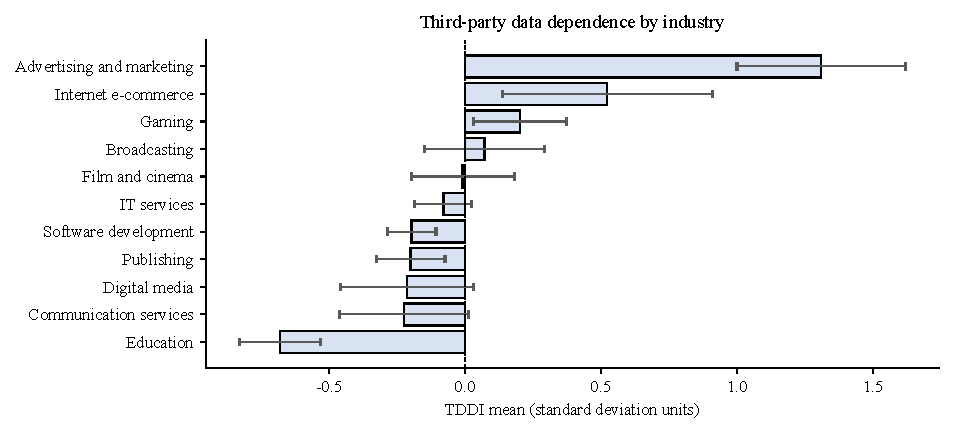
\includegraphics[width=0.95\textwidth]{fig2_tddi_industry.pdf}
\caption{Average TDDI by industry. Bars report the mean TDDI; error bars are standard errors of the mean. The index is standardized to mean zero and unit standard deviation. The sample contains 298 Chinese A-share digital firms; the index is constructed from 2019 annual-report texts.}
\label{fig:tddi}
\end{figure}

\begin{table}[htbp]
\centering
\small
\caption{Construct validity and reliability of the TDDI.}
\label{tab:validity}
\begin{threeparttable}
\begin{tabular}{lccc}
\toprule
 & Pearson correlation & Spearman correlation & Observations \\
\midrule
\multicolumn{4}{l}{Panel A: Correlations with external proxies and a placebo} \\
Selling-expense ratio & -0.005 & 0.119 & 288 \\
Gross margin & 0.031 & 0.120 & 288 \\
ROA & 0.035 & 0.007 & 289 \\
Firm size & 0.116 & 0.188 & 289 \\
Leverage & -0.001 & -0.067 & 289 \\
Generic digitalization & 0.323 & 0.370 & 298 \\
\midrule
\multicolumn{4}{l}{Panel B: Reliability} \\
Split-half correlation (mean of 200 random splits) & 0.677 & & 298 \\
Spearman--Brown corrected correlation & 0.807 & & 298 \\
\bottomrule
\end{tabular}
\begin{tablenotes}[flushleft]
\footnotesize
\item Notes: External proxies are 2019 firm-level averages. The TDDI is constructed from 2019 annual-report texts. The generic digitalization index is the standardized frequency of category F terms and serves as a placebo. The split-half correlation randomly divides the A--D terms into two halves and correlates the resulting indices across firms.
\end{tablenotes}
\end{threeparttable}
\end{table}


\section{Empirical Strategy}
\label{sec:strategy}

\subsection{Baseline Difference-in-Differences}

Let $Y_{it}$ be an outcome for firm $i$ in quarter $t$. Let $\text{HighTDDI}_i$ indicate that firm $i$ is in the top third of the TDDI distribution, and let $\text{Post}_t$ indicate 2021Q3 or later. The baseline specification is
\begin{equation}
Y_{it}=\alpha_i+\lambda_{s(i)t}+\beta\left(\text{HighTDDI}_i\times\text{Post}_t\right)+\Gamma'X_{i,t-1}+\varepsilon_{it},
\label{eq:did}
\end{equation}
where $\alpha_i$ is a firm fixed effect, $\lambda_{s(i)t}$ is an industry-by-quarter fixed effect, and $X_{i,t-1}$ includes lagged firm size, leverage, and the cash ratio. Standard errors are clustered by firm \cite{cameron2015}. Industry-by-quarter fixed effects absorb industry-level shocks, such as the asymmetric effect of the 2020 pandemic on online and offline industries, and the 2022 repricing of technology stocks. Firm fixed effects absorb time-invariant firm characteristics; under heterogeneous treatment effects, two-way fixed-effect estimates require careful interpretation \cite{dechaisemartin2020}. The coefficient $\beta$ measures the differential change in outcomes for high-TDDI firms after the shock, conditional on industry-quarter shocks and observable firm characteristics.

We also estimate a continuous specification:
\begin{equation}
Y_{it}=\alpha_i+\lambda_{s(i)t}+\beta\left(\text{TDDI}_i\times\text{Post}_t\right)+\Gamma'X_{i,t-1}+\varepsilon_{it},
\label{eq:continuous}
\end{equation}
where TDDI is standardized. The continuous specification uses the full cross-section of exposure but imposes linearity \cite{callaway2024}. The binary specification compares the top third with the rest and has a transparent economic interpretation, but depends on the threshold. We report both, with the binary specification as the main design and the continuous specification as a complement. Dose-response bins and a top-versus-bottom comparison test the sensitivity of the results to the threshold.

\subsection{Event Study}

To test parallel trends and trace the time path of the effect, we estimate
\begin{equation}
Y_{it}=\alpha_i+\lambda_{s(i)t}+\sum_{k\neq-1}\beta_k\left(\text{HighTDDI}_i\times\mathbf{1}[t-t_0=k]\right)+\Gamma'X_{i,t-1}+\varepsilon_{it},
\label{eq:event}
\end{equation}
where $t_0$ is 2021Q2, $k=-1$ (2021Q1) is the omitted reference period, and $k$ runs from $-8$ to $10$ (2019Q1 to 2023Q4). The event-study sample starts in 2019; 2018 is used as a burn-in year and is not included in the dynamic plot, which avoids first-year disclosure differences. If the leads are close to zero and the lags turn negative after the shock, the valuation change occurs after the shock rather than before it.

We report the joint test on the leads and the 95\% confidence interval for each event-time coefficient \cite{rambachan2023}. The joint test is interpreted alongside the sign and magnitude of the individual leads. We also report a placebo test with pseudo-shock dates before 2021, which checks whether high-TDDI firms were already on a different trend.

\subsection{Dose-Response and Threshold Sensitivity}

To reduce reliance on a linear functional form, we divide the TDDI into quintiles and estimate
\begin{equation}
Y_{it}=\alpha_i+\lambda_{s(i)t}+\sum_{b=2}^{5}\beta_b\left(\mathbf{1}[\text{TDDI}_i\in Q_b]\times\text{Post}_t\right)+\Gamma'X_{i,t-1}+\varepsilon_{it},
\label{eq:dose}
\end{equation}
where $Q_1$ is the omitted reference group. A monotonic decline in $\beta_b$ indicates a dose-response relationship rather than an effect driven by a single extreme group. We also compare the top third with the bottom third of the TDDI distribution, which uses only the two tails and is therefore less sensitive to the middle group.

\subsection{Placebo Tests and Inference}

We run two placebo tests. First, we assign pseudo-shock dates in 2019Q3 and 2020Q3, restrict the sample to the pre-2021 period, and re-estimate \eqref{eq:did}. If the coefficient is insignificant, the result is not driven by a pre-existing trend or by the pre-pandemic industry cycle. Second, we replace the TDDI with the generic digitalization index and construct a pseudo-treatment variable. If the generic index is insignificant while the TDDI remains significant, the result is not a mechanical reflection of digitalization.

For inference, we report firm-clustered standard errors, two-way clustered standard errors (firm and quarter), and wild cluster bootstrap $p$-values \cite{mackinnon2017}. The baseline wild bootstrap $p$-value is 0.007 (999 replications), consistent with the clustered standard errors. The continuous specification yields a wild bootstrap $p$-value of 0.016. The tables report clustered standard errors; the text reports the more conservative bootstrap results where they differ.

\subsection{Identification and Estimand}

Identification rests on three conditions. First, the TDDI is predetermined: it uses only 2019 annual-report text, which predates ATT and PIPL. Second, conditional parallel trends: absent the privacy shock, high-TDDI and other firms would have followed similar outcome paths after controlling for firm fixed effects, industry-by-quarter fixed effects, and observable characteristics. Third, the shock is exogenous to individual firms: ATT was set by Apple and PIPL by the Chinese legislature, and no single A-share firm could change the timing or content of the rules. The event-study leads and the pseudo-shock tests assess the second condition.

The estimand is the average differential change in valuation and operating outcomes for high-TDDI firms after the 2021 privacy regime. It is not the total value of all data assets, and it is not the social welfare effect of privacy regulation. It is the firm-side market-value exposure to a change in the availability and cost of third-party data. This narrow estimand is what the data can identify, and it is the relevant input for data-asset accounting and for the cost-benefit assessment of privacy rules.

\section{Results}
\label{sec:results}

\subsection{Baseline Estimates}

Table \ref{tab:main} reports the baseline DiD estimates. Panel A compares high-TDDI firms with the rest of the sample. Column (1) shows that high-TDDI firms experience a 0.0917 relative decline in log Tobin's Q after the shock, with a standard error of 0.0343; the estimate is significant at the 1\% level. Relative to the sample mean, this is a 9.2\% valuation discount. Column (2) shows that the level of Tobin's Q declines by 0.3596 (standard error 0.1244). Column (3) shows that gross margin declines by 2.45 percentage points (standard error 1.10), significant at the 5\% level. Columns (4) and (5) show that ROA and the selling-expense ratio change by 0.0004 and $-0.0093$, respectively, and neither effect is significant. The period-expense ratio is also insignificant ($-0.0071$, standard error 0.0091; not tabulated).

Panel B reports the continuous specification. A one-standard-deviation increase in TDDI is associated with a 0.0395 decline in log Tobin's Q (standard error 0.0171), a 0.1700 decline in Tobin's Q (standard error 0.0657), and a 1.24 percentage-point decline in gross margin (standard error 0.53), all significant at the 5\% level. ROA and selling-expense ratios remain insignificant. The continuous and binary specifications point in the same direction and are of comparable magnitude: the binary coefficient is approximately the continuous coefficient scaled by the average TDDI difference between the high group and the rest.

The economic magnitude is substantial. The high-TDDI group had a combined equity market value of RMB 1.72 trillion in 2021Q1. Applying the 9.2\% discount implies a market-value loss of about RMB 203.7 billion (Section 10). This estimate covers only the third-party data channel; it excludes first-party data, algorithms, brands, and network effects. It is therefore a lower bound on the value of the firms' data-related assets, not an estimate of their total data value.

\begin{table}[htbp]
\centering
\small
\setlength{\tabcolsep}{4pt}
\caption{Baseline difference-in-differences estimates.}
\label{tab:main}
\begin{threeparttable}
\begin{tabular}{lccccc}
\toprule
(1) Log Tobin's Q & (2) Tobin's Q & (3) Gross margin & (4) ROA & (5) Selling-expense ratio \\
\midrule
\multicolumn{6}{l}{Panel A: High-TDDI firms (top third)} \\
High TDDI $\times$ Post & -0.0917*** & -0.3596*** & -0.0245** & 0.0004 & -0.0093 \\
 & (0.0343) & (0.1244) & (0.0110) & (0.0023) & (0.0077) \\
\midrule
\multicolumn{6}{l}{Panel B: Continuous TDDI (one-standard-deviation increase)} \\
TDDI $\times$ Post & -0.0395** & -0.1700*** & -0.0124** & -0.0002 & -0.0018 \\
 & (0.0171) & (0.0657) & (0.0053) & (0.0013) & (0.0031) \\
\midrule
Controls & Yes & Yes & Yes & Yes & Yes \\
Firm FE & Yes & Yes & Yes & Yes & Yes \\
Industry $\times$ Quarter FE & Yes & Yes & Yes & Yes & Yes \\
Observations & 6,900 & 6,900 & 6,897 & 6,900 & 6,866 \\
$R^2$ & 0.221 & 0.158 & 0.019 & 0.027 & 0.001 \\
\bottomrule
\end{tabular}
\begin{tablenotes}[flushleft]
\footnotesize
\item Notes: Standard errors clustered by firm are in parentheses. ***, **, and * denote significance at the 1\%, 5\%, and 10\% levels. Post equals one for 2021Q3 and later. High TDDI indicates the top third of the TDDI distribution; the comparison group is the rest of the sample. Controls include lagged firm size, leverage, and the cash ratio. The TDDI is standardized in Panel B.
\end{tablenotes}
\end{threeparttable}
\end{table}


\begin{figure}[htbp]
\centering
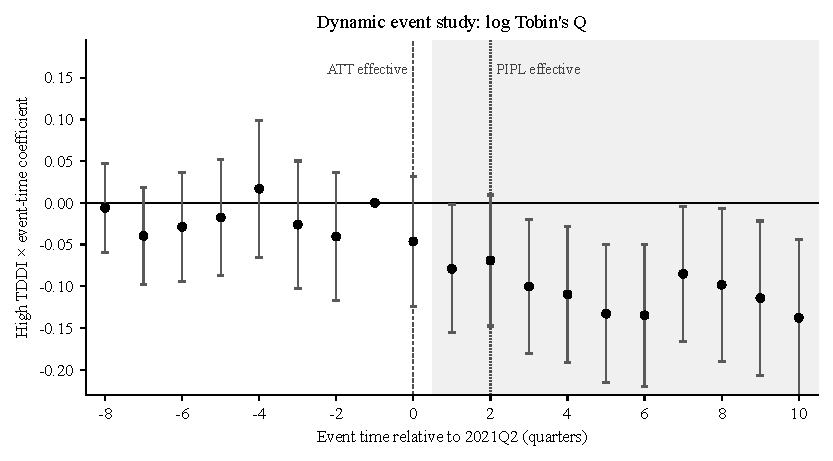
\includegraphics[width=0.95\textwidth]{fig3_event_study.pdf}
\caption{Dynamic event study for log Tobin's Q. Points are coefficients on the interaction between the high-TDDI indicator and event-time dummies; vertical bars are 95\% confidence intervals. The omitted period is 2021Q1 ($k=-1$), shown as a hollow point. Regressions include firm fixed effects, industry-by-quarter fixed effects, and controls. The joint test on the leads yields $p=0.079$. The shaded area is the post-shock period.}
\label{fig:event}
\end{figure}

\subsection{Dynamic Effects}

Figure \ref{fig:event} shows the event-study estimates. The lead coefficients from 2019 to 2020 fluctuate around zero and are individually insignificant. The 2021Q2 coefficient is $-0.046$ and insignificant; the 2021Q3 coefficient is $-0.079$ and significant at the 5\% level. The effect then grows steadily: $-0.100$ in 2022Q1, $-0.133$ in 2022Q3, and $-0.138$ in 2023Q4. The joint test on the leads yields $p=0.079$, which is at the margin of conventional significance. The largest negative lead is about $-0.04$, roughly half the size of the post-shock effect. We therefore interpret the post-shock decline as a break rather than a continuation of a pre-existing trend, and we report placebo and robustness tests in Section 9.4.

The gradual path is consistent with the institutional setting. ATT took effect at the end of Q2 2021, and PIPL took effect in November 2021. Firms needed time to adjust their data collection, advertising technology, and compliance processes. Investors also needed time to reassess the long-run rents from third-party data. The event-study pattern—small and insignificant at the onset, larger and more precise after several quarters—matches this adjustment process.

\subsection{Dose-Response}

Figure \ref{fig:dose} reports the quintile dose-response. Relative to the lowest quintile, the second quintile's coefficient is 0.010 and insignificant, the third is $-0.037$, the fourth is $-0.090$, and the fifth is $-0.090$. The decline occurs mainly between the third and fourth quintiles and then flattens. The highest quintile is significant at the 10\% level, and the top-third versus bottom-third comparison is significant at the 5\% level (Table \ref{tab:hetero}). The pattern indicates a nonlinear dose-response: valuation losses rise sharply once TDDI exceeds the middle of the distribution, and then saturate at the top.

The saturation is economically plausible. Firms in the top quintile are already highly dependent on third-party data; further increases in the text-based index do not necessarily imply proportionally larger exposure. The binary top-third specification captures the economically relevant contrast without imposing a linear relationship across the entire distribution.

\begin{figure}[htbp]
\centering
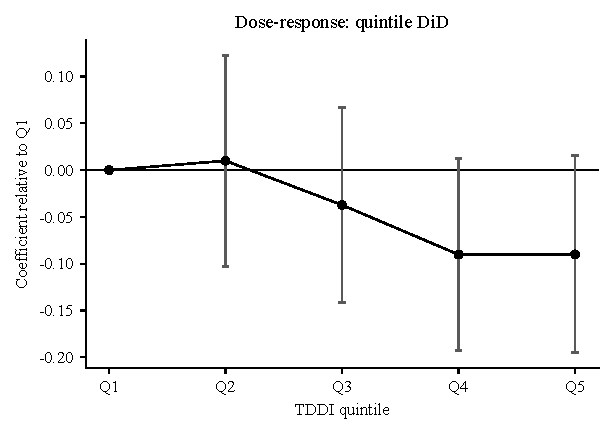
\includegraphics[width=0.72\textwidth]{fig4_dose_response.pdf}
\caption{Dose-response by TDDI quintile. Points are coefficients on the interaction between the quintile indicator and the post-shock dummy; the first quintile is the omitted reference group. Vertical bars are 95\% confidence intervals. Regressions include firm fixed effects, industry-by-quarter fixed effects, and controls.}
\label{fig:dose}
\end{figure}

\subsection{Placebo Tests}

We assign pseudo-shock dates in 2019Q3 and 2020Q3 and restrict the sample to the pre-2021 period. The coefficients on high TDDI interacted with the pseudo-shock are $-0.032$ (standard error 0.033) and $-0.032$ (standard error 0.032), respectively, and neither is significant. Replacing the TDDI with the generic digitalization index yields a coefficient of $-0.021$ (standard error 0.019), also insignificant. In a horse race that includes both high TDDI and high generic digitalization, the TDDI coefficient is $-0.075$ (standard error 0.036) and the generic digitalization coefficient is $-0.040$ (standard error 0.035), with only the former significant. The results are therefore not driven by a pre-existing trend or by a generic digitalization narrative.

\section{Mechanisms and Heterogeneity}
\label{sec:mechanism}

\subsection{Valuation versus Profitability}

Table \ref{tab:main} shows a combination that is central to the interpretation: gross margin declines by 2.45 percentage points after the shock, while ROA and expense ratios do not change significantly. This pattern implies that the privacy shock compresses the profitability of revenue rather than the scale of operating costs. A natural explanation is that third-party data support pricing, targeting, and conversion. When the data become less available, the same revenue requires more acquisition effort or generates lower conversion, which lowers gross margin. Firms simultaneously cut low-efficiency advertising and administrative spending, which keeps ROA stable in the short run. The decline in data rents therefore appears in the quality of revenue rather than in the level of expenses.

The selling-expense ratio is consistent with this interpretation. If the shock operated mainly through higher customer-acquisition costs, the selling-expense ratio should rise. The estimated effect is $-0.0093$ (standard error 0.0077), negative and insignificant. Firms did not simply spend more on advertising; they adjusted the composition of spending, reduced low-efficiency channels, or moderated acquisition intensity. A falling gross margin without a rising selling-expense ratio points to a decline in data-driven pricing and matching, not to a pure cost shock.

\subsection{B2B versus B2C Firms}

Table \ref{tab:hetero} reports the heterogeneity results. B2B data-service firms—IT services, software, and communication services—experience a 14.2\% decline in log Tobin's Q (standard error 4.4\%), significant at the 1\% level. Consumer internet firms—advertising, gaming, e-commerce, digital media, film, publishing, broadcasting, and education—experience a 2.0\% decline (standard error 5.2\%), which is not significant. The difference is economically large: the point estimate for B2B firms is about seven times that for consumer firms, and a pooled interaction model yields a difference significant at the 10\% level ($p=0.107$). The top-third versus bottom-third comparison yields a 10.7\% decline in log Tobin's Q, a 0.329 decline in Tobin's Q, and a 3.41 percentage-point decline in gross margin.

This is the paper's central mechanism result. Third-party data dependence is not evenly distributed across digital firms. B2B data-service firms obtain data through external procurement, client authorization, cross-organizational sharing, and project-based delivery. PIPL's consent, minimization, and sharing rules directly raise the compliance cost of these activities, while ATT weakens their ability to provide cross-app attribution and targeted delivery to clients. Consumer internet firms own accounts, transaction records, first-party apps, and membership relationships; first-party data can substitute for part of the lost third-party data. Their valuations are therefore less sensitive to the privacy shock.

The result also clarifies what a ``data asset'' is. Data are not homogeneous bits. A unit of first-party data and a unit of third-party data have different substitutability under privacy regulation, and therefore different value. Treating all digital firms as a single data-asset category obscures the structural difference between B2B and B2C firms. The TDDI identifies this difference because it measures dependence on external data, not the level of digitalization.

\subsection{First-Party Data Capability}

Table \ref{tab:hetero} also reports the FPDCI split. High-FPDCI firms experience a 12.6\% decline in log Tobin's Q (standard error 5.5\%), while low-FPDCI firms experience a 9.5\% decline (standard error 5.3\%); both are significant, and the point estimate for the high-FPDCI group is slightly larger. The App-exposure split is similarly muted: high-app-exposure firms decline by 8.7\% (standard error 4.4\%), and low-app-exposure firms decline by 9.4\% (standard error 6.7\%). These results do not support a simple substitution story in which first-party data fully insulate firms from the shock.

A more plausible interpretation is that first-party data capability and third-party data dependence coexist. High-FPDCI firms are often data-intensive firms: they own user accounts and transaction data, but they also purchase external data to extend coverage, improve models, and conduct cross-platform advertising. When privacy regulation tightens, first-party data can buffer part of the shock, but it cannot replace the breadth and cross-domain reach of third-party data. The two data types are complements as much as substitutes. This finding qualifies the popular view that private-domain traffic is a safe harbor under privacy regulation: private data are valuable, but they do not make firms immune to the contraction of the third-party data ecosystem.

\begin{table}[htbp]
\centering
\small
\caption{Heterogeneity by firm type, app exposure, and first-party data capability.}
\label{tab:hetero}
\begin{threeparttable}
\begin{tabular}{lccc}
\toprule
 & Log Tobin's Q & Tobin's Q & Gross margin \\
\midrule
B2B firms & -0.1424*** (0.0438) & -0.4902*** (0.1637) & -0.0339*** (0.0121) \\
Consumer firms & -0.0197 (0.0523) & -0.1556 (0.1849) & -0.0095 (0.0198) \\
Low app exposure & -0.0942 (0.0671) & -0.2640 (0.1996) & -0.0155 (0.0192) \\
High app exposure & -0.0866* (0.0444) & -0.3972** (0.1714) & -0.0191 (0.0156) \\
Low FPDCI & -0.0952* (0.0525) & -0.4518** (0.1923) & 0.0006 (0.0179) \\
High FPDCI & -0.1261** (0.0553) & -0.3572* (0.2064) & -0.0505*** (0.0189) \\
\bottomrule
\end{tabular}
\begin{tablenotes}[flushleft]
\footnotesize
\item Notes: Each cell reports the coefficient on High TDDI $\times$ Post, with firm-clustered standard errors in parentheses. B2B firms include IT services, software development, and communication services. Consumer firms include advertising, gaming, e-commerce, digital media, film, publishing, broadcasting, and education. App exposure and FPDCI are split at the median. The top-third versus bottom-third comparison is reported in the text.
\end{tablenotes}
\end{threeparttable}
\end{table}


\subsection{Robustness}

Table \ref{tab:robust} reports 11 robustness checks. First, replacing the baseline TDDI with a narrow measure based only on category A (third-party data acquisition) yields a coefficient of $-0.0824$ (standard error 0.0355), significant at the 5\% level. Second, replacing the TDDI with the generic digitalization index yields $-0.0214$ (standard error 0.0193), which is insignificant. Third, in a horse race with both high TDDI and high generic digitalization, the TDDI coefficient is $-0.0748$ (standard error 0.0363) and the generic coefficient is $-0.0396$ (standard error 0.0349), with only the former significant. Fourth, excluding 2020 yields $-0.0932$. Fifth, restricting the sample to firms with at least 20 quarters yields $-0.0976$. Sixth, excluding firms in the top 1\% of assets yields $-0.0945$. Seventh, controlling for a 2020--2021 pandemic interaction yields $-0.1027$. Eighth, two-way clustering by firm and quarter yields a standard error of 0.0339 and leaves the significance unchanged. Ninth, winsorizing at the 5th and 95th percentiles yields $-0.0777$. Tenth, the top-third versus bottom-third comparison yields $-0.1067$. The wild cluster bootstrap $p$-value for the baseline coefficient is 0.007. All checks point in the same direction: the result is not driven by a single measure, subsample, extreme value, or clustering choice.

\begin{table}[htbp]
\centering
\small
\caption{Robustness checks for log Tobin's Q.}
\label{tab:robust}
\begin{threeparttable}
\begin{tabular}{lcccc}
\toprule
 & Coefficient & Standard error & $p$-value & Observations \\
\midrule
Baseline: high TDDI & -0.0917*** & (0.0343) & 0.007 & 6,900 \\
Narrow TDDI measure & -0.0824** & (0.0355) & 0.020 & 6,900 \\
Placebo: generic digitalization & -0.0214 & (0.0193) & 0.268 & 6,900 \\
Horse race: TDDI and generic digitalization & -0.0748** & (0.0363) & 0.039 & 6,900 \\
Excluding 2020 & -0.0932*** & (0.0339) & 0.006 & 5,733 \\
Balanced panel (at least 20 quarters) & -0.0976*** & (0.0344) & 0.005 & 6,458 \\
Excluding the top 1\% by assets & -0.0945*** & (0.0351) & 0.007 & 6,831 \\
Controlling for the 2020--2021 pandemic interaction & -0.1027*** & (0.0396) & 0.009 & 6,900 \\
Two-way clustering (firm and quarter) & -0.0917*** & (0.0339) & 0.007 & 6,900 \\
Winsorizing at the 5th and 95th percentiles & -0.0777** & (0.0329) & 0.018 & 6,900 \\
Top third versus bottom third & -0.1067** & (0.0443) & 0.016 & 4,631 \\
\bottomrule
\end{tabular}
\begin{tablenotes}[flushleft]
\footnotesize
\item Notes: All columns use log Tobin's Q as the dependent variable and include firm fixed effects, industry-by-quarter fixed effects, and controls. The wild cluster bootstrap $p$-value for the baseline coefficient is 0.007 (999 replications). The generic digitalization index is the standardized frequency of category F terms; it should be insignificant if the TDDI captures a distinct construct.
\end{tablenotes}
\end{threeparttable}
\end{table}


\section{The Data Risk Exposure}
\label{sec:value}

\subsection{From Coefficients to Market Value}

The baseline coefficient can be translated into an implied change in firm value. By the definition of Tobin's Q, $Q_{it}=(M_{it}+D_{it})/A_{it}$, where $M$ is equity market value and $D$ is total liabilities. For small changes, the proportional change in log Tobin's Q is approximately the proportional change in the sum of equity value and liabilities. For a high-TDDI firm $i$, using 2021Q1 as the base period, the implied market-value loss is
\begin{equation}
\widehat{\Delta M}_i=\hat{\beta}\left(M_{i,2021Q1}+D_{i,2021Q1}\right),
\label{eq:dmv}
\end{equation}
where $\hat{\beta}=-0.0917$ is the binary coefficient in column (1) of Table \ref{tab:main}. Summing $\widehat{\Delta M}_i$ over the 100 high-TDDI firms gives the sample-level data risk exposure. The confidence interval uses the standard error of $\hat{\beta}$ times $\pm1.96$ and the same base-period value.

Table \ref{tab:value} reports the results by industry. The total implied market-value loss for high-TDDI firms is about RMB 203.7 billion, with a 95\% confidence interval of RMB 54.7--352.8 billion. Software development has the largest loss (RMB 61.5 billion), followed by communication services (RMB 35.2 billion), advertising and marketing (RMB 25.7 billion), IT services (RMB 23.1 billion), and gaming (RMB 16.0 billion). The ranking differs from the TDDI ranking because absolute losses depend on both exposure intensity and market value. Advertising has the highest average TDDI, but its high-TDDI firms are smaller on average, so the absolute loss is lower than in software and communication services.

\begin{figure}[htbp]
\centering
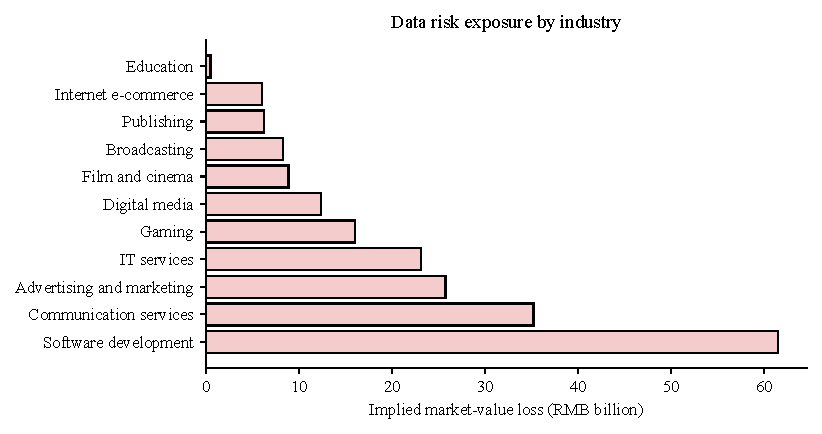
\includegraphics[width=0.9\textwidth]{fig5_value_by_industry.pdf}
\caption{Implied market-value loss of high-TDDI firms by industry. Bars are the implied loss from applying the baseline log Tobin's Q coefficient ($-0.0917$) to the sum of 2021Q1 equity market value and liabilities. Units are RMB billion. The sample contains the 100 high-TDDI firms.}
\label{fig:value}
\end{figure}

\subsection{Interpreting the Estimate}

The RMB 203.7 billion figure is a data risk exposure, not the total value of data assets. It has three interpretations. First, it is a firm-side private cost: the privacy regime reduces the expected rents from third-party data, and the market adjusts valuations accordingly. It does not include the consumer privacy benefits or the welfare effects of the regulation. Second, it covers a narrow asset class: third-party tracking, advertising, and data-service data. First-party data, algorithms, brands, network effects, and user relationships are outside the calculation. Third, it is a market revaluation of future rents, not the historical cost of acquiring data or the replacement cost of data infrastructure.

For data-asset accounting, the estimate provides an operational benchmark. Current data-asset recognition focuses on internally generated data resources and uses cost or income approaches. The risk exposure from third-party data dependence is not yet a standard accounting item. Our results show that third-party data dependence is a measurable, priceable, and industry-specific risk factor. For regulators, the magnitude indicates that the cost of privacy regulation is not borne only by consumers; B2B data-service firms and data-dependent software and communication firms bear a substantial adjustment cost. For investors, the TDDI can serve as an ex ante observable risk indicator for data-intensive firms.

The estimate can also be read as a lower bound on the value of the affected data. It captures only the portion of data rents that the market expected to be lost under the 2021 regime. If firms adapt by building first-party data, using privacy-enhancing technologies, or changing their advertising mix, the long-run loss may be smaller. If the shock also reduced the option value of future data-driven products, the total value of the affected data would be larger. The point estimate is a benchmark, and the confidence interval reflects the uncertainty in the valuation coefficient.

\begin{table}[htbp]
\centering
\small
\small
\setlength{\tabcolsep}{3pt}
\caption{Implied market-value loss of high-TDDI firms by industry.}
\label{tab:value}
\begin{threeparttable}
\begin{tabular}{lccccc}
\toprule
Industry & Firms & Market value (RMB bn) & Implied loss (RMB bn) & 95\% lower & 95\% upper \\
\midrule
Software development & 20 & 630.9 & 61.5 & 16.5 & 106.5 \\
Communication services & 4 & 144.3 & 35.2 & 9.4 & 61.0 \\
Advertising and marketing & 17 & 236.4 & 25.7 & 6.9 & 44.5 \\
IT services & 23 & 199.9 & 23.1 & 6.2 & 40.0 \\
Gaming & 11 & 149.6 & 16.0 & 4.3 & 27.8 \\
Digital media & 3 & 122.8 & 12.3 & 3.3 & 21.4 \\
Film and cinema & 6 & 67.0 & 8.9 & 2.4 & 15.4 \\
Broadcasting & 5 & 60.8 & 8.3 & 2.2 & 14.3 \\
Publishing & 5 & 49.9 & 6.2 & 1.7 & 10.7 \\
Internet e-commerce & 5 & 57.9 & 6.0 & 1.6 & 10.4 \\
Education & 1 & 4.6 & 0.5 & 0.1 & 0.8 \\
\midrule
Total & 100 & 1724.2 & 203.7 & 54.7 & 352.8 \\
\bottomrule
\end{tabular}
\begin{tablenotes}[flushleft]
\footnotesize
\item Notes: The implied loss applies the baseline log Tobin's Q coefficient ($-0.0917$) to the sum of 2021Q1 equity market value and liabilities. Confidence intervals use the coefficient standard error times $\pm1.96$. The sample contains the 100 high-TDDI firms. The estimate is the market-value exposure to the privacy shock, not the total value of all data assets.
\end{tablenotes}
\end{threeparttable}
\end{table}


\section{Discussion}
\label{sec:discussion}

\subsection{Privacy Regulation as a Valuation Shock}

The results show that the 2021 privacy regime changed the valuation of Chinese digital firms. The average effect is negative for high-TDDI firms, but the distribution of the effect is uneven. B2B data-service firms lose value, while consumer internet firms with first-party data do not. This pattern is consistent with the view that privacy regulation redistributes rents across business models rather than simply reducing the total amount of data in the economy.

The comparison with prior work is instructive. Studies of the GDPR document average effects on web traffic, advertising, and firm performance \cite{goldberg2024,aridor2020}. Studies of ATT document effects on e-commerce, app monetization, and the app ecosystem \cite{aridor2024,kesler2023,cheyre2024}. These designs compare regulated and unregulated markets, or exposed and unexposed users. Our design compares firms within the same regulated market and uses predetermined text-based exposure. The results show that the cross-sectional distribution of exposure is economically important: average effects can mask large losses in data-service segments and negligible effects in first-party-data segments.

The B2B--B2C contrast also speaks to the JTAER literature on privacy regulation and platform competition. Recent work shows that privacy regulation affects retailer resilience through customer-acquisition dependence and traffic architecture \cite{chen2026}. Our results complement this finding by showing that the valuation effect is concentrated in firms that sell data-intensive services to other firms. Privacy regulation operates not only through consumer consent but also through the business-to-business data supply chain.

\subsection{Implications for Data-Asset Accounting}

Data-asset accounting currently focuses on the recognition and measurement of internally generated data resources. The results suggest that third-party data dependence is a distinct risk factor. Two firms with the same book assets and the same reported revenue can have different exposure to privacy regulation because their data inputs differ. A TDDI-style measure can be constructed from public disclosures, validated with reliability tests, and used as an auxiliary risk indicator in valuation and disclosure.

The RMB 203.7 billion estimate provides a benchmark for the firm-side cost of the 2021 regime. It is not a social cost, because it excludes consumer privacy benefits. It is also not the total value of data, because it covers only third-party data. It is, however, a useful order of magnitude for policy analysis: the adjustment cost is concentrated in a few industries and in a relatively small number of firms.

\subsection{Implications for Firms and Investors}

For firms, the results imply that third-party data dependence should be managed as a valuation risk. B2B data-service firms need to reassess the compliance cost of data procurement, client authorization, and cross-organizational sharing. Consumer firms with first-party data are less exposed, but they are not immune: first-party data did not fully buffer the shock in our sample. Building first-party data capability is valuable, but it is not a complete substitute for external data.

For investors, the TDDI provides an ex ante risk ranking. A text-based index can be computed before a regulatory shock, updated annually, and combined with industry and market-value data to estimate exposure. This is particularly relevant for data-intensive small and medium firms, whose data practices are less visible to analysts than those of large platforms.

\subsection{Scope of the Estimate}

The estimate applies to the 2021 privacy regime and to Chinese A-share digital firms. It captures the combined effect of ATT and PIPL, which overlap in time and operate through related margins. The TDDI is a text-based proxy for data dependence, and the sample covers an important segment of the digital economy. Within this scope, the estimated exposure is large and uneven across business models.

\section{Conclusions}
\label{sec:conclusion}

Data are a core production factor of the digital economy, but their asset value is difficult to observe. This paper turns the broad question ``what are data worth?'' into a narrow empirical question: when a privacy regime raises the cost of third-party data, how much market value do exposed firms lose? We answer this question using the 2021 ATT and PIPL shock, a text-based TDDI constructed from 2019 annual reports, and a firm-quarter panel of 298 Chinese A-share digital firms from 2018Q1 to 2023Q4.

The evidence supports H1, H2, and H3. The main findings are threefold. First, high-TDDI firms experience a 9.2\% relative decline in log Tobin's Q and a 2.45 percentage-point decline in gross margin after the shock, while ROA and selling-expense ratios do not change significantly. Second, the effect is concentrated in B2B data-service firms, which decline by 14.2\%, while consumer internet firms are not significantly affected. Third, the implied market-value loss for high-exposure firms is about RMB 203.7 billion, with a 95\% confidence interval of RMB 54.7--352.8 billion. The FPDCI split does not support a buffering role for first-party data (H4); instead, first-party data capability and third-party data dependence appear to coexist.

The paper contributes a replicable measure of third-party data dependence, a valuation estimate for a privacy-regime shock, and a data risk exposure that can inform data-asset accounting and privacy policy. The B2B--B2C contrast shows that data assets are not homogeneous: first-party data and third-party data have different substitutability under privacy regulation, and the firms that intermediate external data bear a disproportionate share of the adjustment cost.

Three extensions follow naturally. First, the TDDI can be applied to other markets and other privacy regimes, which would test the external validity of the exposure measure. Second, linking the index to firm-level data flows, app-level tracking, or advertising outcomes would provide a more direct validation of the mechanism. Third, a dynamic model of first-party data investment would clarify whether the observed valuation loss is permanent or is offset by adaptation over time. These extensions would deepen the understanding of how data assets are priced in the digital economy.


\section*{Author Contributions}
Conceptualization, A.N. and C.N.; methodology, A.N.; software, A.N.; validation, A.N. and C.N.; formal analysis, A.N.; data curation, A.N.; writing---original draft preparation, A.N.; writing---review and editing, C.N.; visualization, A.N.; supervision, C.N. All authors have read and agreed to the published version of the manuscript.

\section*{Funding}
This research received no external funding.

\section*{Institutional Review Board Statement}
Not applicable.

\section*{Informed Consent Statement}
Not applicable.

\section*{Data Availability Statement}
The financial and market data are available from the public databases described in Section 5. The annual-report texts are available from the CNINFO and Eastmoney disclosure platforms. The constructed panel and replication code are available from the corresponding author upon reasonable request.

\section*{Conflicts of Interest}
The authors declare no conflicts of interest.

\appendix
\setcounter{table}{0}
\renewcommand{\thetable}{A\arabic{table}}

\section{Variable Definitions}
\label{app:vars}

Table \ref{tab:vars} lists the variables used in the analysis, their definitions, and their sources. Financial variables are quarterly. Flow variables are differenced from year-to-date cumulative values, and ratio variables are winsorized at the 1st and 99th percentiles.

\begin{table}[htbp]
\centering
\small
\caption{Variable definitions and data sources.}
\label{tab:vars}
\begin{threeparttable}
\begin{tabular}{p{3.2cm}p{8.4cm}p{3.2cm}}
\toprule
Variable & Definition & Source \\
\midrule
TDDI & Equal-weighted average of the A--D term frequencies, log-transformed and standardized & 2019 annual reports; authors' construction \\
FPDCI & Log-standardized frequency of first-party data terms & 2019 annual reports; authors' construction \\
Tobin's Q & (Equity market value + total liabilities) / total assets & Eastmoney \\
Log Tobin's Q & Natural logarithm of Tobin's Q & Authors' calculation \\
ROA & Net profit attributable to the parent / total assets & Eastmoney \\
Gross margin & (Operating revenue $-$ operating costs) / operating revenue & Eastmoney \\
Selling-expense ratio & Selling expenses / operating revenue & Eastmoney \\
Period-expense ratio & (Selling + administrative expenses) / operating revenue & Eastmoney \\
Firm size & Natural logarithm of total assets & Authors' calculation \\
Leverage & Total liabilities / total assets & Authors' calculation \\
Cash ratio & Cash holdings / total assets & Authors' calculation \\
High TDDI & Top third of the TDDI distribution & Authors' construction \\
Post & 2021Q3 and later & Authors' construction \\
\bottomrule
\end{tabular}
\begin{tablenotes}[flushleft]
\footnotesize
\item Notes: Financial variables are quarterly. Flow variables are differenced from year-to-date cumulative values. Ratio variables are winsorized at the 1st and 99th percentiles.
\end{tablenotes}
\end{threeparttable}
\end{table}


\section{TDDI Lexicon}
\label{app:lexicon}

Table \ref{tab:lexicon} lists the six constructs of the TDDI lexicon and representative terms. The longest-match rule ensures that each character span is counted once. Frequencies are normalized per 10,000 characters. The complete term list is in the replication code.

\begin{table}[htbp]
\centering
\small
\caption{TDDI lexicon: constructs and representative terms.}
\label{tab:lexicon}
\begin{threeparttable}
\begin{tabular}{p{3.2cm}p{10.0cm}p{1.2cm}}
\toprule
Construct & Representative terms & Terms \\
\midrule
A. Third-party data acquisition & third-party data, purchased data, data procurement, data supplier, data transaction, data sharing, data interface, data source, data fusion & 33 \\
B. Third-party traffic and advertising & traffic purchase, customer acquisition cost, ad buying, advertising placement, precision marketing, programmatic advertising, information-flow advertising, ad network, app distribution & 37 \\
C. User profiling and tracking & user profile, tag system, cross-app, cross-device, device identifier, IDFA, OAID, targeted placement, personalized recommendation, audience package & 30 \\
D. Platform dependence & third-party platform, open platform, app store, iOS, WeChat mini-program, Douyin, Kuaishou, Xiaohongshu, Ocean Engine, Alimama & 26 \\
E. First-party data capability & owned data, first-party data, private-domain traffic, membership system, user community, WeCom, CRM, data middle platform, CDP & 28 \\
F. Generic digitalization (placebo) & digital transformation, cloud computing, big data, artificial intelligence, Internet of Things, blockchain, 5G, industrial internet, large language model & 18 \\
\bottomrule
\end{tabular}
\begin{tablenotes}[flushleft]
\footnotesize
\item Notes: The longest-match rule ensures that each character span is counted once. Frequencies are normalized per 10,000 characters. The complete list is in the replication code.
\end{tablenotes}
\end{threeparttable}
\end{table}


\section{Event-Study Coefficients}
\label{app:event}

Table \ref{tab:event} reports the full event-study coefficients underlying Figure \ref{fig:event}. The omitted period is 2021Q1. The joint test on the leads yields $p=0.079$.

\begin{table}[htbp]
\centering
\small
\caption{Full event-study coefficients for log Tobin's Q.}
\label{tab:event}
\begin{threeparttable}
\begin{tabular}{lcc}
\toprule
Event time $k$ & Coefficient & Standard error \\
\midrule
-8 & -0.0059 & 0.0273 \\
-7 & -0.0396 & 0.0296 \\
-6 & -0.0288 & 0.0331 \\
-5 & -0.0176 & 0.0357 \\
-4 & 0.0169 & 0.0420 \\
-3 & -0.0261 & 0.0389 \\
-2 & -0.0404 & 0.0392 \\
0 & -0.0462 & 0.0399 \\
1 & -0.0790** & 0.0392 \\
2 & -0.0690* & 0.0400 \\
3 & -0.1002** & 0.0407 \\
4 & -0.1097*** & 0.0414 \\
5 & -0.1329*** & 0.0423 \\
6 & -0.1348*** & 0.0435 \\
7 & -0.0851** & 0.0413 \\
8 & -0.0981** & 0.0469 \\
9 & -0.1140** & 0.0471 \\
10 & -0.1378*** & 0.0480 \\
\bottomrule
\end{tabular}
\begin{tablenotes}[flushleft]
\footnotesize
\item Notes: The dependent variable is log Tobin's Q. Event time is measured in quarters relative to 2021Q2; $k=-1$ is the omitted reference period. All regressions include firm fixed effects, industry-by-quarter fixed effects, and controls. The joint test on the leads yields $p=0.079$.
\end{tablenotes}
\end{threeparttable}
\end{table}



\begin{thebibliography}{99}

\bibitem{jones2020}
Jones, C.I.; Tonetti, C. Nonrivalry and the Economics of Data. \textit{American Economic Review} \textbf{2020}, \textit{110}, 2819--2858. \url{https://doi.org/10.1257/aer.20191330}.

\bibitem{farboodi2020}
Farboodi, M.; Veldkamp, L. Long-Run Growth of Financial Data Technology. \textit{American Economic Review} \textbf{2020}, \textit{110}, 2485--2523. \url{https://doi.org/10.1257/aer.20171349}.

\bibitem{bergemann2019}
Bergemann, D.; Bonatti, A. Markets for Information: An Introduction. \textit{Annual Review of Economics} \textbf{2019}, \textit{11}, 85--107. \url{https://doi.org/10.1146/annurev-economics-080315-015439}.

\bibitem{oecd2022}
OECD. The Value of Data in Digital-Based Business Models: Measurement and Economic Policy Implications. \textit{OECD Economics Department Working Papers} \textbf{2022}. \url{https://doi.org/10.1787/d960a10c-en}.

\bibitem{goldberg2024}
Goldberg, S.G.; Johnson, G.A.; Shriver, S.K. Regulating Privacy Online: An Economic Evaluation of the GDPR. \textit{American Economic Journal: Economic Policy} \textbf{2024}, \textit{16}, 325--358. \url{https://doi.org/10.1257/pol.20210309}.

\bibitem{apple2020}
Apple Inc. User Privacy and Data Use. 2020. Available online: \url{https://developer.apple.com/app-store/user-privacy-and-data-use/} (accessed on 27 October 2026).

\bibitem{pipl2021}
Standing Committee of the National People's Congress. Personal Information Protection Law of the People's Republic of China. 2021. Available online: \url{https://www.gov.cn/xinwen/2021-08/20/content_5632486.htm} (accessed on 27 October 2026).

\bibitem{aridor2024}
Aridor, G.; Che, Y.-K.; Hollenbeck, B.; Kaiser, M.; McCarthy, D. Evaluating the Impact of Privacy Regulation on E-Commerce Firms: Evidence from Apple's App Tracking Transparency. \textit{Management Science} \textbf{2024}, forthcoming. \url{https://doi.org/10.1287/mnsc.2024.06600}.

\bibitem{kesler2023}
Kesler, R. The Impact of Apple's App Tracking Transparency on App Monetization. SSRN Working Paper No. 4090786, 2023. \url{https://papers.ssrn.com/sol3/papers.cfm?abstract_id=4090786}.

\bibitem{cheyre2024}
Cheyre, C.; Leyden, B.T.; Baviskar, S.; Acquisti, A. Did Apple's App Tracking Transparency Framework Harm the App Ecosystem? Knight-Georgetown Institute Working Paper, 2024. \url{https://kgi.georgetown.edu/wp-content/uploads/2024/12/Cristobal-Cheyre.pdf}.

\bibitem{gentzkow2019}
Gentzkow, M.; Kelly, B.; Taddy, M. Text as Data. \textit{Journal of Economic Literature} \textbf{2019}, \textit{57}, 535--574. \url{https://doi.org/10.1257/jel.20181020}.

\bibitem{loughran2011}
Loughran, T.; McDonald, B. When Is a Liability Not a Liability? Textual Analysis, Dictionaries, and 10-Ks. \textit{Journal of Finance} \textbf{2011}, \textit{66}, 35--65. \url{https://doi.org/10.1111/j.1540-6261.2010.01625.x}.

\bibitem{baker2016}
Baker, S.R.; Bloom, N.; Davis, S.J. Measuring Economic Policy Uncertainty. \textit{Quarterly Journal of Economics} \textbf{2016}, \textit{131}, 1593--1636. \url{https://doi.org/10.1093/qje/qjw024}.

\bibitem{jin2026}
Jin, L.; Cai, X.; Wang, J. Digital Transformation and Enterprise Operating Costs: Evidence from Chinese A-Share Listed Firms. \textit{Sustainability} \textbf{2026}, \textit{18}, 4189. \url{https://doi.org/10.3390/su18094189}.

\bibitem{dechaisemartin2020}
de Chaisemartin, C.; D'Haultf{\oe}uille, X. Two-Way Fixed Effects Estimators with Heterogeneous Treatment Effects. \textit{American Economic Review} \textbf{2020}, \textit{110}, 2964--2996. \url{https://doi.org/10.1257/aer.20181169}.

\bibitem{rambachan2023}
Rambachan, A.; Roth, J. An Honest Approach to Parallel Trends. Working Paper, 2023. \url{https://www.jonathandroth.com/assets/files/HonestParallelTrends_Main_July21.pdf}.

\bibitem{callaway2024}
Callaway, B.; Goodman-Bacon, A.; Sant'Anna, P.H.C. Difference-in-Differences with a Continuous Treatment. NBER Working Paper No. 32117, 2024. \url{https://www.nber.org/papers/w32117}.

\bibitem{mackinnon2017}
MacKinnon, J.G.; Webb, M.D. Wild Bootstrap Inference for Wildly Different Cluster Sizes. \textit{Journal of Applied Econometrics} \textbf{2017}, \textit{32}, 233--254. \url{https://doi.org/10.1002/jae.2508}.

\bibitem{chen2026}
Chen, Q.; Chen, R. Privacy Regulation and Online Retailer Resilience: The Roles of Customer-Acquisition Dependence and Traffic Architecture. \textit{Journal of Theoretical and Applied Electronic Commerce Research} \textbf{2026}, \textit{21}, 388. \url{https://doi.org/10.3390/jtaer21110388}.

\bibitem{ma2025}
Ma, Y.; Li, Z.; He, L. Data Elements Marketization and Corporate Investment Efficiency: Causal Inference via Double Machine Learning. \textit{Systems} \textbf{2025}, \textit{13}, 609. \url{https://doi.org/10.3390/systems13070609}.

\bibitem{acquisti2016}
Acquisti, A.; Taylor, C.; Wagman, L. The Economics of Privacy. \textit{Journal of Economic Literature} \textbf{2016}, \textit{54}, 442--492. \url{https://doi.org/10.1257/jel.54.2.442}.

\bibitem{tucker2014}
Tucker, C.E. Social Networks, Personalized Advertising, and Privacy Controls. \textit{Journal of Marketing Research} \textbf{2014}, \textit{51}, 546--562. \url{https://doi.org/10.1509/jmr.10.0355}.

\bibitem{johnson2020}
Johnson, G.A.; Shriver, S.K.; Du, S. Consumer Privacy Choice in Online Advertising: Who Opts Out and at What Cost to Industry? \textit{Marketing Science} \textbf{2020}, \textit{39}, 33--51. \url{https://doi.org/10.1287/mksc.2019.1198}.

\bibitem{li2026}
Li, B.; Wang, C.; Wu, Y.; Chen, B.; Hao, Z. Which Privacy Policy Works, Opt-In Requirement or Inference Regulation? A Game-Theoretic Analysis of Privacy Policies in E-Commerce. \textit{Journal of Theoretical and Applied Electronic Commerce Research} \textbf{2026}, \textit{21}, 184. \url{https://doi.org/10.3390/jtaer21060184}.

\bibitem{kang2025}
Kang, J.; Lan, J.; Huang, S.; Chen, L. Effects of Privacy Regulatory Protection on Users' Data Sharing in Mobile Apps. \textit{Journal of Theoretical and Applied Electronic Commerce Research} \textbf{2025}, \textit{20}, 153. \url{https://doi.org/10.3390/jtaer20030153}.

\bibitem{lin2021}
Lin, X.; Huang, X.; Liu, S.; Li, Y.; Luo, H.; Yu, S. Social Welfare Analysis under Different Levels of Consumers' Privacy Regulation. \textit{Journal of Theoretical and Applied Electronic Commerce Research} \textbf{2021}, \textit{16}, 2943--2964. \url{https://doi.org/10.3390/jtaer16070161}.

\bibitem{zhang2026}
Zhang, Y.; Shen, Y.; Zhong, W. Consumer Privacy Control and Targeted Advertisement on Content Platforms: Resolving the Privacy--Personalization Paradox in Data-Driven Marketing. \textit{Journal of Theoretical and Applied Electronic Commerce Research} \textbf{2026}, \textit{21}, 328. \url{https://doi.org/10.3390/jtaer21090328}.

\bibitem{song2025}
Song, Y.; Xu, C. Marketization of Data Elements and Corporate Green Innovation: Evidence from the Establishment of Data Trading Platforms in China. \textit{Sustainability} \textbf{2025}, \textit{17}, 10980. \url{https://doi.org/10.3390/su172410980}.

\bibitem{acquisti2015}
Acquisti, A.; Brandimarte, L.; Loewenstein, G. Privacy and Human Behavior in the Age of Information. \textit{Science} \textbf{2015}, \textit{347}, 509--514. \url{https://doi.org/10.1126/science.aaa1465}.

\bibitem{goldfarb2012}
Goldfarb, A.; Tucker, C. Shifts in Privacy Concerns. \textit{American Economic Review} \textbf{2012}, \textit{102}, 349--353. \url{https://doi.org/10.1257/aer.102.3.349}.

\bibitem{bleier2015}
Bleier, A.; Eisenbeiss, M. Personalized Online Advertising Effectiveness: The Interplay of What, When, and Where. \textit{Marketing Science} \textbf{2015}, \textit{34}, 669--688. \url{https://doi.org/10.1287/mksc.2015.0930}.

\bibitem{boerman2017}
Boerman, S.C.; Kruikemeier, S.; Zuiderveen Borgesius, F.J. Online Behavioral Advertising: A Literature Review and Research Agenda. \textit{Journal of Advertising} \textbf{2017}, \textit{46}, 363--376. \url{https://doi.org/10.1080/00913367.2017.1339368}.

\bibitem{casadesus2015}
Casadesus-Masanell, R.; Hervas-Drane, A. Competing with Privacy. \textit{Management Science} \textbf{2015}, \textit{61}, 229--246. \url{https://doi.org/10.1287/mnsc.2014.2023}.

\bibitem{acquisti2005}
Acquisti, A.; Varian, H.R. Conditioning Prices on Purchase History. \textit{Marketing Science} \textbf{2005}, \textit{24}, 367--381. \url{https://doi.org/10.1287/mksc.1040.0103}.

\bibitem{ichihashi2020}
Ichihashi, S. Online Privacy and Information Disclosure by Consumers. \textit{American Economic Review} \textbf{2020}, \textit{110}, 569--595. \url{https://doi.org/10.1257/aer.20181052}.

\bibitem{bonatti2020}
Bonatti, A.; Cisternas, G. Consumer Scores and Price Discrimination. \textit{Review of Economic Studies} \textbf{2020}, \textit{87}, 750--791. \url{https://doi.org/10.1093/restud/rdz046}.

\bibitem{culnan1999}
Culnan, M.J.; Armstrong, P.K. Information Privacy Concerns, Procedural Fairness, and Impersonal Trust: An Empirical Investigation. \textit{Organization Science} \textbf{1999}, \textit{10}, 104--115. \url{https://doi.org/10.1287/orsc.10.1.104}.

\bibitem{dinev2006}
Dinev, T.; Hart, P. An Extended Privacy Calculus Model for E-Commerce Transactions. \textit{Information Systems Research} \textbf{2006}, \textit{17}, 61--80. \url{https://doi.org/10.1287/isre.1060.0080}.

\bibitem{malhotra2004}
Malhotra, N.K.; Kim, S.S.; Agarwal, J. Internet Users' Information Privacy Concerns (IUIPC): The Construct, the Scale, and a Causal Model. \textit{Information Systems Research} \textbf{2004}, \textit{15}, 336--355. \url{https://doi.org/10.1287/isre.1040.0032}.

\bibitem{nissenbaum2009}
Nissenbaum, H. \textit{Privacy in Context: Technology, Policy, and the Integrity of Social Life}; Stanford University Press: Stanford, CA, USA, 2009.

\bibitem{samuelson2000}
Samuelson, P. Privacy as Intellectual Property? \textit{Stanford Law Review} \textbf{2000}, \textit{52}, 1125--1173. \url{https://doi.org/10.2307/1229511}.

\bibitem{hermalin2006}
Hermalin, B.E.; Katz, M.L. Privacy, Property Rights and Efficiency: The Economics of Privacy as Secrecy. \textit{Quantitative Marketing and Economics} \textbf{2006}, \textit{4}, 209--239. \url{https://doi.org/10.1007/s11129-005-9004-7}.

\bibitem{aridor2020}
Aridor, G.; Che, Y.-K.; Salz, T. The Economic Consequences of Data Privacy Regulation: Empirical Evidence from GDPR. SSRN Working Paper No. 3522845, 2020. \url{https://papers.ssrn.com/sol3/papers.cfm?abstract_id=3522845}.

\bibitem{wang2023}
Wang, Z.; Yuan, C.; Li, X. Evolutionary Analysis of the Regulation of Data Abuse in Digital Platforms. \textit{Systems} \textbf{2023}, \textit{11}, 188. \url{https://doi.org/10.3390/systems11040188}.

\bibitem{mihaylova2026}
Mihaylova, Z. Governing the Privacy--Personalization Tension in AI-Driven Marketing Platforms: An Integrative Framework for Customer Data Platforms. \textit{Platforms} \textbf{2026}, \textit{4}, 21. \url{https://doi.org/10.3390/platforms4040021}.

\bibitem{dsl2021}
Standing Committee of the National People's Congress. Data Security Law of the People's Republic of China. 2021. Available online: \url{https://www.gov.cn/xinwen/2021-06/11/content_5616919.htm} (accessed on 27 October 2026).

\bibitem{cameron2015}
Cameron, A.C.; Miller, D.L. A Practitioner's Guide to Cluster-Robust Inference. \textit{Journal of Human Resources} \textbf{2015}, \textit{50}, 317--372. \url{https://doi.org/10.3368/jhr.50.2.317}.

\end{thebibliography}

\end{document}
